\documentclass[11pt]{article}

\usepackage[margin=1in]{geometry}
\usepackage{amsmath,amssymb}
\usepackage{booktabs}
\usepackage{enumitem}
\usepackage{longtable}
\usepackage{graphicx}
\usepackage{caption}
\usepackage{xcolor}
\usepackage{setspace}
\setstretch{1.15}            % 15% more space between lines; try 1.2 for more
\usepackage[parfill]{parskip} % blank space between paragraphs instead of indents
\usepackage[colorlinks=true,linkcolor=blue!50!black,citecolor=blue!50!black,urlcolor=blue!50!black]{hyperref}

% Marks anything the team still has to produce with its own code or sources.
\newcommand{\todo}[1]{\textcolor{red!70!black}{\textbf{[TODO:} #1\textbf{]}}}

\newcommand{\rE}{\mathbf{r}_E}
\newcommand{\vE}{\mathbf{v}_E}
\newcommand{\gEI}{\gamma_{\mathrm{EI}}}
\newcommand{\bu}{\mathbf{u}}
\newcommand{\bff}{\mathbf{f}}

\title{How Accurate Must a Free-Return Translunar Burn Be,\\ and What Does Correcting an Injection Error Cost?}
\author{AE 370 Group Project 1 \\ Zohair Hasson, Jammir Aloya, Akhil Boyapati, Jeehyung Yoo}
\date{Fall 2026}

\begin{document}
\maketitle

% =====================================================================
\section{Premise}
\label{sec:premise}
% =====================================================================

\subsection{Motivation}

A \emph{free-return trajectory} carries a spacecraft from Earth, around the Moon, and back to Earth without any further major propulsive maneuver. If the main engine fails after translunar injection (TLI), the Moon's gravity alone bends the trajectory home, which makes free return the default abort-safe design for crewed lunar missions.

Apollo~13 shows both why free return matters and why it is not sufficient on its own. A midcourse correction on the second day had moved the spacecraft off free return onto a \emph{hybrid} trajectory to reach the Fra Mauro landing site, so when the oxygen tank failed the spacecraft was not on a path that would return it to Earth~\cite{nasa_apollo13}. At 61\,h\,30\,min mission elapsed time (MET), the crew fired the Lunar Module descent engine for 34\,s to re-establish free return~\cite{nasa_apollo13}. Further corrections followed after the lunar flyby, including a 14.8\,s burn at 105\,h\,18\,min MET to fine-tune the reentry path~\cite{nasa_apollo13}. Mission Control described the acceptable entry corridor as approximately $-5.25^\circ$ to $-7.4^\circ$ of flight-path angle at entry interface, and targeted the final correction to $-6.52^\circ$~\cite{afj_day5}.

Returning to Earth's vicinity is therefore not enough: the spacecraft must reach the atmosphere within a narrow band of \emph{entry flight-path angle} $\gEI$. Too shallow, and the capsule skips off the atmosphere; too steep, and deceleration and heating exceed crew and vehicle limits. Modern capsules such as Orion define their entry corridor in terms of $\gEI$ and the vehicle's lift-to-drag ratio~\cite{rea_orion}; on Artemis~I, Orion reached entry interface at $\gEI = -5.66^\circ$ and an inertial speed of $36{,}063$\,ft/s ($\approx 10.99$\,km/s)~\cite{rea_artemis1}, inside the Apollo corridor.

The lunar flyby strongly amplifies small errors in the TLI burn. Simulating our nominal free return (defined below) shows that, to first order, a $1$\,mm/s error in TLI magnitude changes $\gEI$ by about $0.14^\circ$, and a $1$\,s error in burn timing changes it by about $5.7^\circ$. The entire $2.15^\circ$ corridor therefore corresponds to only about $15$\,mm/s of TLI magnitude and about $0.4$\,s of burn timing: accuracy at the millimeter-per-second and sub-second level, beyond what an engine can deliver open-loop, which is why midcourse corrections exist. This project quantifies those accuracy requirements and the propellant cost of correcting an imperfect burn.

\subsection{Research questions}

\begin{enumerate}[label=\textbf{Q\arabic*.}, leftmargin=2.5em]
  \item \textbf{Injection accuracy.} How sensitive is the entry flight-path angle $\gEI$ to errors in (a)~TLI burn magnitude and (b)~TLI burn timing? What are the largest errors in each that keep $\gEI$ within the corridor $-7.4^\circ \le \gEI \le -5.25^\circ$~\cite{afj_day5}?
  \item \textbf{Correction cost.} When a TLI error places the spacecraft outside the corridor, how large an impulsive midcourse correction $\Delta v_c$ is required to restore $\gEI = -6.52^\circ$, and how does that cost depend on the correction time $t_c$? In particular, is it cheaper to correct before or after the lunar flyby, and by how much?
\end{enumerate}

\noindent\textbf{Hypothesis.} We expect the allowable TLI errors to be on the order of millimeters per second and fractions of a second, and the correction cost to depend strongly on $t_c$, with the lunar flyby marking a clear transition. The numerical study is designed to confirm or refute both.

\subsection{Model and assumptions}

We model the spacecraft with the \emph{planar circular restricted three-body problem} (CR3BP)~\cite{szebehely}, under the following assumptions:
\begin{enumerate}[leftmargin=2em]
  \item Earth and Moon are point masses on circular orbits about their common barycenter.
  \item The spacecraft's mass is negligible and does not perturb Earth or Moon.
  \item Motion is confined to the Earth--Moon orbital plane; the Moon's orbital inclination is neglected.
  \item Solar gravity, solar radiation pressure, and Earth oblateness ($J_2$) are neglected.
  \item All burns are impulsive (instantaneous velocity changes).
  \item There is no atmosphere. $\gEI$ is evaluated where the vacuum trajectory crosses the entry-interface altitude, consistent with its use as a targeting criterion in mission design.
\end{enumerate}

\subsection{The initial value problem}

Figure~\ref{fig:geometry} shows the geometry: the spacecraft departs a low Earth parking orbit, swings behind the Moon, and returns to cross the entry interface, where the entry flight-path angle $\gEI$ is measured.

\begin{figure}[t]
\centering
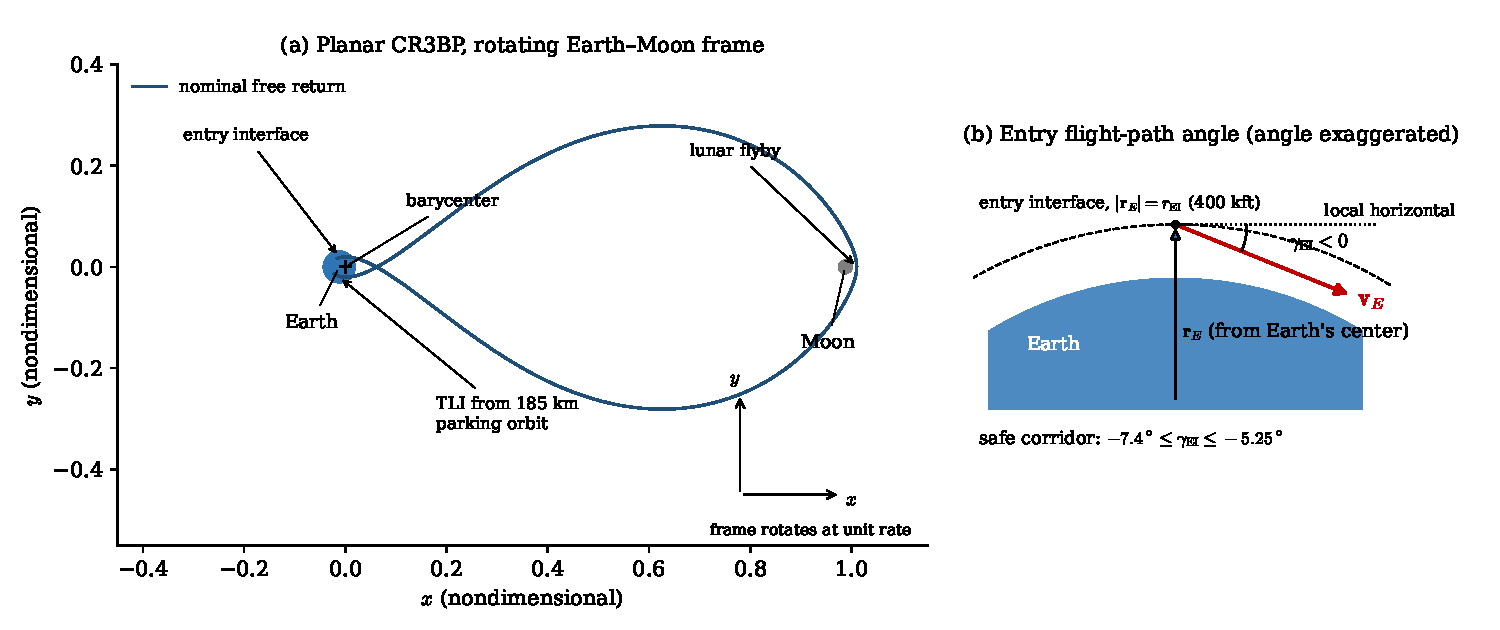
\includegraphics[width=\textwidth]{figures/premise_geometry.pdf}
\caption{(a) The nominal free return in the rotating Earth--Moon frame, computed with our RK4 implementation (Earth and Moon not to scale). (b) Definition of the entry flight-path angle $\gEI$ at entry interface: the angle between the Earth-relative inertial velocity $\vE$ and the local horizontal, negative when descending.}
\label{fig:geometry}
\end{figure}

\paragraph{Nondimensionalization.} Lengths, times, and velocities are scaled as in Table~\ref{tab:units}. Earth lies at $(-\mu, 0)$ and the Moon at $(1-\mu, 0)$ in a frame rotating with the Earth--Moon line at unit angular rate.

\begin{table}[h]
\centering
\caption{Nondimensional units and problem constants.}
\label{tab:units}
\begin{tabular}{@{}llll@{}}
\toprule
Quantity & Symbol & Dimensional & Nondimensional \\
\midrule
Length unit (Earth--Moon distance) & $L$ & $384{,}400$ km & 1 \\
Time unit (inverse orbital rate) & $T$ & $4.3425$ days & 1 \\
Velocity unit & $V = L/T$ & $1.0246$ km/s & 1 \\
Mass parameter & $\mu = m_M/(m_E+m_M)$ & --- & $0.012154$ \\
Earth radius & $R_E$ & $6{,}378.165$ km & $0.016593$ \\
Moon radius & $R_M$ & $1{,}737.4$ km & $0.004520$ \\
Parking orbit radius (185 km alt.) & $r_0$ & $6{,}563.2$ km & $0.017074$ \\
Entry interface radius (400{,}000 ft alt.) & $r_{\mathrm{EI}}$ & $6{,}500.1$ km & $0.016910$ \\
\bottomrule
\end{tabular}
\end{table}

\noindent The time unit is not set independently: the nondimensional equations assume $G(m_E + m_M) = L^3/T^2$, so $T = \sqrt{L^3/G(m_E+m_M)}$ with $m_E = 5.9722\times10^{24}$\,kg and $m_M = 7.3477\times10^{22}$\,kg. The entry-interface altitude of 400{,}000\,ft follows the convention used for Orion~\cite{rea_artemis1}.

\paragraph{Governing equations.} With state $\bu = [x,\ y,\ v_x,\ v_y]^T$ in the rotating frame,
\begin{equation}
\label{eq:cr3bp}
\begin{aligned}
\dot x &= v_x, \\
\dot y &= v_y, \\
\dot v_x &= 2v_y + x - \frac{(1-\mu)(x+\mu)}{r_1^3} - \frac{\mu(x-1+\mu)}{r_2^3}, \\
\dot v_y &= -2v_x + y - \frac{(1-\mu)\,y}{r_1^3} - \frac{\mu\,y}{r_2^3},
\end{aligned}
\end{equation}
where
\begin{equation}
r_1 = \sqrt{(x+\mu)^2 + y^2}, \qquad r_2 = \sqrt{(x-1+\mu)^2 + y^2}
\end{equation}
are the distances to Earth and Moon. The $\pm 2v$ terms are the Coriolis acceleration and the bare $x$, $y$ terms the centrifugal acceleration. Equation~\eqref{eq:cr3bp} is a coupled, nonlinear, autonomous IVP,
\begin{equation}
\dot{\bu} = \bff(\bu), \qquad \bu(0) = \bu_0 .
\end{equation}

\paragraph{Initial condition: TLI from a parking orbit.} The spacecraft starts on a circular, prograde 185\,km parking orbit at angle $\varphi$ from the Earth--Moon line and performs a tangential TLI burn of magnitude $\Delta v$ (dimensional, km/s):
\begin{equation}
\label{eq:ic}
\begin{aligned}
x_0 &= -\mu + r_0\cos\varphi, \qquad y_0 = r_0\sin\varphi, \\
v_c &= \sqrt{\frac{1-\mu}{r_0}} + \frac{\Delta v}{V}, \\
v_{x,0} &= -v_c \sin\varphi + y_0, \qquad v_{y,0} = v_c\cos\varphi - (x_0+\mu).
\end{aligned}
\end{equation}
The final line converts the inertial velocity to the rotating frame via $\mathbf{v}_{\mathrm{rot}} = \mathbf{v}_{\mathrm{in}} - \boldsymbol{\omega}\times\mathbf{r}$, including Earth's motion about the barycenter. Burn \emph{timing} maps to $\varphi$: a timing error $\delta t$ shifts the burn location by $\delta\varphi = n_{\mathrm{LEO}}\,\delta t$, where $n_{\mathrm{LEO}} = \sqrt{(1-\mu)/r_0^3}$ is the parking-orbit angular rate.

\paragraph{Nominal trajectory and parameters.} The nominal free return is found numerically. A scan over $\Delta v$ and $\varphi$ locates a free-return family near $\varphi = 4.12$\,rad; holding $\varphi$ fixed, bisection on $\Delta v$ (\texttt{scripts/retarget\_nominal.py}) gives $\Delta v = 3.144030$\,km/s, for which $\gEI = -6.520^\circ$. Just below this value the return skips past the atmosphere (at $\Delta v = 3.1440$\,km/s the vacuum perigee is $147$\,km), and $0.5$\,m/s above it the entry is already $-28.7^\circ$. The nominal passes $6{,}947$\,km above the lunar surface $3.77$ days after TLI and reaches entry interface $7.56$ days after TLI at $10.99$\,km/s, the same as Orion's measured entry speed on Artemis~I~\cite{rea_artemis1}. Table~\ref{tab:params} lists the parameters the investigation varies and the quantities it measures.

\begin{table}[h]
\centering
\caption{Investigated parameters and measured outputs.}
\label{tab:params}
\small
\begin{tabular}{@{}llll@{}}
\toprule
Parameter & Symbol & Nominal / range & Question \\
\midrule
TLI magnitude error & $\delta(\Delta v)$ & $0$; swept over $\pm 20$ mm/s & Q1a \\
TLI timing error & $\delta t$ ($\delta\varphi = n_{\mathrm{LEO}}\delta t$) & $0$; swept over $\pm 2$ s & Q1b \\
Injection error to be corrected & $\delta(\Delta v)$ & e.g.\ $\pm 1$ m/s & Q2 \\
Correction time & $t_c$ & 15--20 values, TLI to $\approx$1 day before EI & Q2 \\
Correction magnitude & $\Delta v_c$ & solved for, along $\vE/|\vE|$ & Q2 \\
\midrule
\multicolumn{4}{@{}l}{\emph{Held fixed:} $\mu$, $r_0$, $r_{\mathrm{EI}}$, nominal $\Delta v$ and $\varphi$, corridor $[-7.4^\circ, -5.25^\circ]$, target $-6.52^\circ$} \\
\multicolumn{4}{@{}l}{\emph{Measured:} $\gEI$ (primary); perilune altitude, time of flight, $\Delta v_c$} \\
\bottomrule
\end{tabular}
\end{table}

\paragraph{Events and derived quantities.} Let $\rE = (x+\mu,\ y)$ be the Earth-relative position and
\begin{equation}
\vE = (v_x - y,\ \ v_y + x + \mu)
\end{equation}
the Earth-relative inertial velocity. \emph{Entry interface} is the first crossing of $|\rE| = r_{\mathrm{EI}}$ after the lunar flyby, where the entry flight-path angle is
\begin{equation}
\label{eq:gamma}
\gEI = \arcsin\!\left(\frac{\rE\cdot\vE}{|\rE|\,|\vE|}\right).
\end{equation}
A run is flagged as a \emph{lunar impact} if $r_2 < R_M$, and as \emph{no return} if it fails to reach entry interface within 3 time units ($\approx 13$ days). Along any coasting arc the \emph{Jacobi constant}
\begin{equation}
\label{eq:jacobi}
C = 2\Omega - \left(v_x^2 + v_y^2\right), \qquad
\Omega = \tfrac{1}{2}\left(x^2+y^2\right) + \frac{1-\mu}{r_1} + \frac{\mu}{r_2},
\end{equation}
is conserved; it changes only at impulsive burns.

\subsection{Why numerical methods are required}

The CR3BP is non-integrable: no general closed-form solution exists~\cite{szebehely}. The nominal free return, the sensitivity of $\gEI$ to injection errors, and the correction cost all depend on the full nonlinear passage through the Earth--Moon system, including the lunar flyby that drives the error amplification. Patched-conic approximations treat the flyby as an instantaneous switch between two-body problems; they can provide a rough nominal trajectory, but not the sensitivities at the heart of this project. Every answer to Q1 and Q2 therefore comes from numerically integrating Eq.~\eqref{eq:cr3bp}. Analytical solutions are used only to verify the implementation (Section~\ref{sec:verification}).

% =====================================================================
\section{Numerical method}
\label{sec:method}
% =====================================================================

\subsection{The scheme}

We advance Eq.~\eqref{eq:cr3bp} with the classical fourth-order Runge--Kutta method (RK4) at a fixed time step $\Delta t$:
\begin{equation}
\label{eq:rk4}
\begin{aligned}
\mathbf{k}_1 &= \bff(\bu_k), &
\mathbf{k}_2 &= \bff\!\left(\bu_k + \tfrac{\Delta t}{2}\mathbf{k}_1\right), \\
\mathbf{k}_3 &= \bff\!\left(\bu_k + \tfrac{\Delta t}{2}\mathbf{k}_2\right), &
\mathbf{k}_4 &= \bff\!\left(\bu_k + \Delta t\,\mathbf{k}_3\right), \\
\bu_{k+1} &= \bu_k + \tfrac{\Delta t}{6}\left(\mathbf{k}_1 + 2\mathbf{k}_2 + 2\mathbf{k}_3 + \mathbf{k}_4\right).
\end{aligned}
\end{equation}

\subsection{Error and stability properties}

\paragraph{Truncation error.} RK4 has local truncation error $O(\Delta t^5)$ and global error $O(\Delta t^4)$. \todo{derive in the language of Lectures 10--11: Taylor-expand Eq.~\eqref{eq:rk4} and match terms through $\Delta t^4$.}

\paragraph{Absolute stability.} Applying Eq.~\eqref{eq:rk4} to the test equation $\dot u = \lambda u$ gives $u_{k+1} = R(w)\,u_k$ with $w = \lambda\Delta t$ and
\begin{equation}
R(w) = 1 + w + \frac{w^2}{2} + \frac{w^3}{6} + \frac{w^4}{24}.
\end{equation}
On the imaginary axis, $w = iy$,
\begin{equation}
|R(iy)|^2 = 1 - \frac{y^6}{72} + \frac{y^8}{576},
\end{equation}
so $|R(iy)| \le 1$ if and only if $y^2 \le 8$, i.e.\ $|y| \le 2\sqrt{2} \approx 2.83$. By contrast, forward Euler gives $|1+iy|^2 = 1 + y^2 > 1$ for every $y \neq 0$, and the stability region of AB2 touches the imaginary axis only at the origin; AB3 and AB4 cover it only up to $|y| \approx 0.72$ and $0.43$.

\paragraph{Eigenvalues along the trajectory.} Figure~\ref{fig:stiffness}(a) shows the largest Jacobian eigenvalue magnitude along the nominal free return. It peaks at the low-Earth ends of the trip, where the eigenvalues are $\pm\sqrt{2}\,n$ (real) and $\pm i\,n$, with $n$ the local orbital rate; at the parking orbit $|\lambda|_{\max} = 630$. The negative-real and imaginary eigenvalues must lie inside the stability region. The positive-real one is the physical divergence of neighbouring trajectories, the same mechanism that amplifies TLI errors, and must be resolved accurately rather than damped. At the study time step (Section~\ref{sec:verification}) $|\lambda|\Delta t = 0.019$, far inside the region (Figure~\ref{fig:stiffness}b).

\begin{figure}[t]
\centering
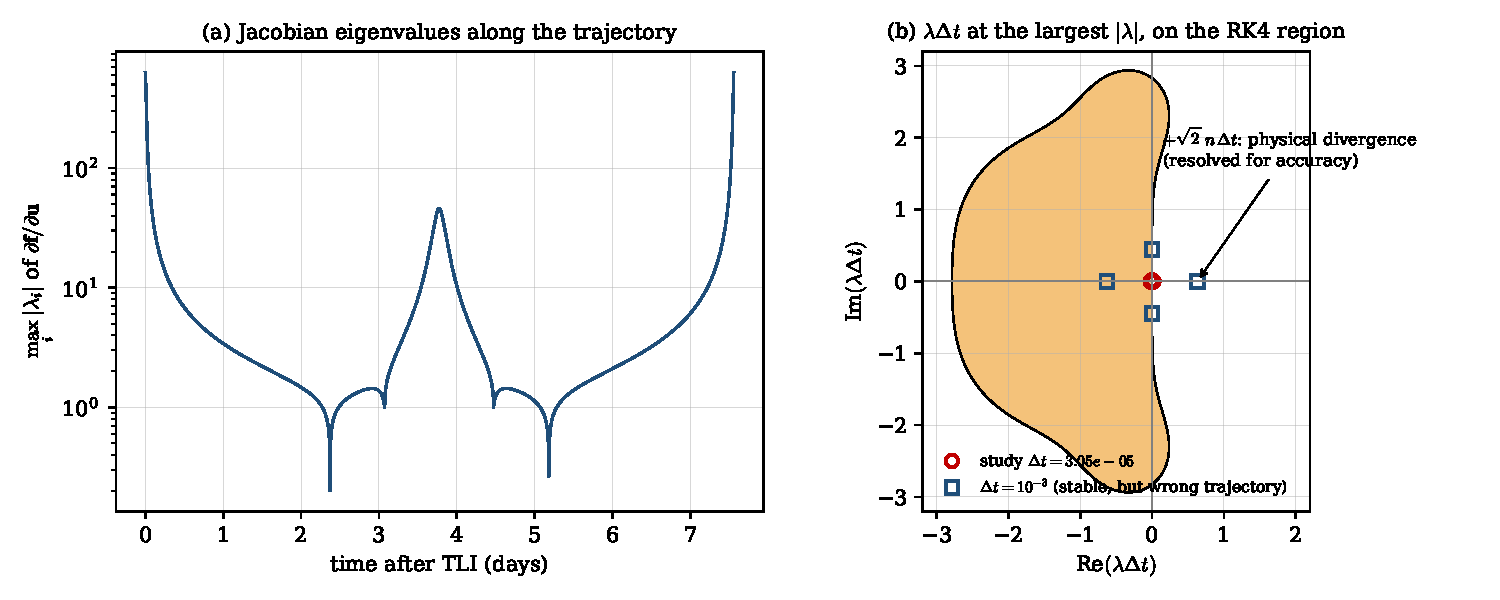
\includegraphics[width=\textwidth]{figures/stiffness_along_trajectory.pdf}
\caption{(a) Largest Jacobian eigenvalue magnitude along the nominal free return; the central peak is the lunar flyby. (b) $\lambda\Delta t$ at the state with the largest $|\lambda|$, on the RK4 stability region, for the study time step and for $\Delta t = 10^{-3}$. Even at $\Delta t = 10^{-3}$ every decaying and oscillatory mode is stable, yet that run never returns to Earth: the step is limited by accuracy, not stability.}
\label{fig:stiffness}
\end{figure}

\subsection{Justification: accuracy, stability, and cost}

\begin{itemize}[leftmargin=2em]
  \item \textbf{Accuracy.} The required $\gEI$ accuracy is a small fraction of a $2.15^\circ$ corridor, and the sensitivities in Q1 must be resolved at the sub-mm/s level. A fourth-order method reaches this accuracy with orders of magnitude fewer steps than a first- or second-order method.
  \item \textbf{Stability.} Near Earth the motion has oscillatory modes $\pm i\,n$ on the imaginary axis. RK4's stability region contains the segment $|\lambda\Delta t| \le 2\sqrt{2}$ of that axis; forward Euler's and AB2's contain none of it, so both would artificially amplify orbital oscillations at any $\Delta t$.
  \item \textbf{Not stiff, so explicit is appropriate.} The Jacobian eigenvalues are largest near Earth, but there the solution itself varies on the same short timescale. The step is limited by \emph{accuracy}, not stability, so an implicit method (backward Euler, trapezoid, BDF2) would add a nonlinear solve every step with no benefit. Figure~\ref{fig:stiffness}(b) shows this directly: at $\Delta t = 10^{-3}$, $|\lambda\Delta t| = 0.63$ for the real modes and $0.45$ for the oscillatory ones, well inside the region, yet the trajectory never returns to Earth.
  \item \textbf{One step, not multistep.} A midcourse correction changes the velocity instantly, and locating entry interface needs a partial step. A one-step method handles both directly; a multistep method such as AB4 would have to restart its history after every burn. (At our time step $|\lambda|\Delta t \approx 0.02$ is also inside AB4's region, so stability alone would not rule AB4 out.)
  \item \textbf{Cost, and why adaptive stepping is not used.} The problem is multi-scale: the parking-orbit period is $0.0141$ time units against a trip of $1.740$. Adaptive step-size control would therefore reduce function evaluations. However, fixed-step RK4 at the study time step $\Delta t = 3.05\times 10^{-5}$ ($11.4$\,s) takes about $2$\,s per run in plain Python, and the full study requires a few hundred runs. Adaptive control would add an error estimator, step-rejection logic, and a less transparent convergence study, without changing the answers.
\end{itemize}

\subsection{Algorithm: advancing from $t_k$ to $t_{k+1}$}

\begin{enumerate}[leftmargin=2em]
  \item Evaluate $\mathbf{k}_1,\dots,\mathbf{k}_4$ from $\bu_k$ and form $\bu_{k+1}$ via Eq.~\eqref{eq:rk4}.
  \item \textbf{Entry-interface event.} If, after the flyby, $|\rE| - r_{\mathrm{EI}}$ changes sign between $\bu_k$ and $\bu_{k+1}$, find $\tau \in (0, \Delta t)$ by root-finding (Brent's method) such that a single RK4 step of length $\tau$ from $\bu_k$ lands exactly on $|\rE| = r_{\mathrm{EI}}$, then evaluate Eq.~\eqref{eq:gamma}. Locating the event with an RK4 step preserves $O(\Delta t^4)$ accuracy; taking the minimum over sampled steps would introduce an $O(\Delta t^2)$ error.
  \item \textbf{Lunar impact.} If $r_2 < R_M$, flag the run and stop.
  \item \textbf{Midcourse correction.} At the step $k$ with $t_k$ nearest $t_c$, add $\Delta v_c$ along $\vE/|\vE|$ to the velocity components of $\bu_k$ before stepping. The position is unchanged, so the same vector is added to the rotating-frame velocity.
\end{enumerate}

\subsection{Targeting}

Retargeting the nominal (find $\Delta v$ such that $\gEI = -6.52^\circ$) and sizing corrections (find $\Delta v_c$ such that $\gEI = -6.52^\circ$) are scalar root-finding problems wrapped around our RK4 integrator. We use bisection or \texttt{scipy.optimize.brentq}; root-finders are permitted, external time integrators are not.

% =====================================================================
\section{Implementation and verification}
\label{sec:verification}
% =====================================================================

\subsection{Verification against independent results}

\begin{table}[h]
\centering
\caption{Verification tests.}
\label{tab:verify}
\begin{tabular}{@{}p{3.6cm}p{5.4cm}p{5.2cm}@{}}
\toprule
Test & What it checks & Pass criterion \\
\midrule
Two-body exact solution ($\mu = 0$) & Integrator and rotating-frame terms coded correctly & Error vs.\ exact solution decreases as $O(\Delta t^4)$ \\
Published periodic orbit (JPL) & Full three-body equations, including every Moon term & Closure error after one period decreases as $O(\Delta t^4)$ \\
Jacobi constant & Conservation law of the coasting CR3BP & $\max_t |C(t) - C(0)|$ decreases as $O(\Delta t^4)$ \\
Convergence rate & Method achieves its theoretical order & Observed order $\approx 4$ in the asymptotic range \\
Event-location order & $\gEI$ inherits fourth-order accuracy & $\gEI$ error decreases as $O(\Delta t^4)$ \\
\bottomrule
\end{tabular}
\end{table}

\paragraph{Two-body exact solution.} Setting $\mu = 0$ in Eq.~\eqref{eq:cr3bp} places Earth at the origin with unit gravitational parameter, so the system reduces to Kepler motion viewed from a frame rotating at unit rate, for which the inertial solution is known exactly. We choose an ellipse with perigee radius $r_p = r_0$ and eccentricity $e = 0.97$, close to the shape of the translunar ellipse, giving
\begin{equation}
a = \frac{r_p}{1-e} = 0.5691, \qquad b = a\sqrt{1-e^2}, \qquad n = a^{-3/2}, \qquad P = \frac{2\pi}{n} = 2.698 .
\end{equation}
Measuring time from perigee, the eccentric anomaly $E$ satisfies Kepler's equation $nt = E - e\sin E$, which we solve with Newton's method,
\begin{equation}
E_{j+1} = E_j - \frac{E_j - e\sin E_j - nt}{1 - e\cos E_j}, \qquad E_0 = \pi,
\end{equation}
to $|E_{j+1}-E_j| < 10^{-15}$. The inertial state follows from
\begin{equation}
\mathbf{r}_{\mathrm{in}} = \begin{bmatrix} a(\cos E - e) \\ b\sin E \end{bmatrix}, \qquad
\mathbf{v}_{\mathrm{in}} = \frac{n}{1 - e\cos E}\begin{bmatrix} -a\sin E \\ b\cos E \end{bmatrix},
\end{equation}
and is rotated into the CR3BP frame by
\begin{equation}
\mathbf{r}_{\mathrm{rot}} = \mathsf{R}(-t)\,\mathbf{r}_{\mathrm{in}}, \qquad
\mathbf{v}_{\mathrm{rot}} = \mathsf{R}(-t)\,\mathbf{v}_{\mathrm{in}} + \begin{bmatrix} y_{\mathrm{rot}} \\ -x_{\mathrm{rot}} \end{bmatrix}, \qquad
\mathsf{R}(-t) = \begin{bmatrix} \cos t & \sin t \\ -\sin t & \cos t \end{bmatrix},
\end{equation}
where the second term in $\mathbf{v}_{\mathrm{rot}}$ comes from differentiating the time-dependent rotation. The integration starts from the exact perigee state $\bu_0 = [\,r_p,\ 0,\ 0,\ v_p - r_p\,]^T$ with $v_p = \sqrt{(1+e)/r_p} = 10.74$ ($11.0$\,km/s), the same speed as TLI and lunar-return entry, and calls the same right-hand-side function used for all results with $\mu = 0$. We measure $\varepsilon(\Delta t) = \|\mathbf{r}_{\mathrm{num}}(t_f) - \mathbf{r}_{\mathrm{exact}}(t_f)\|_2$ at $t_f = P/2$ (apogee) and $t_f = P$ (back at perigee), with $\Delta t = t_f/N$ so that the march lands exactly on $t_f$. Figure~\ref{fig:kepler} shows observed orders $4.02$--$4.21$. At every $\Delta t$ the full-orbit error is about $36\times$ the half-orbit error, because most of the error accumulates during the perigee passage; this is why perigee sets the time step.

\begin{figure}[t]
\centering
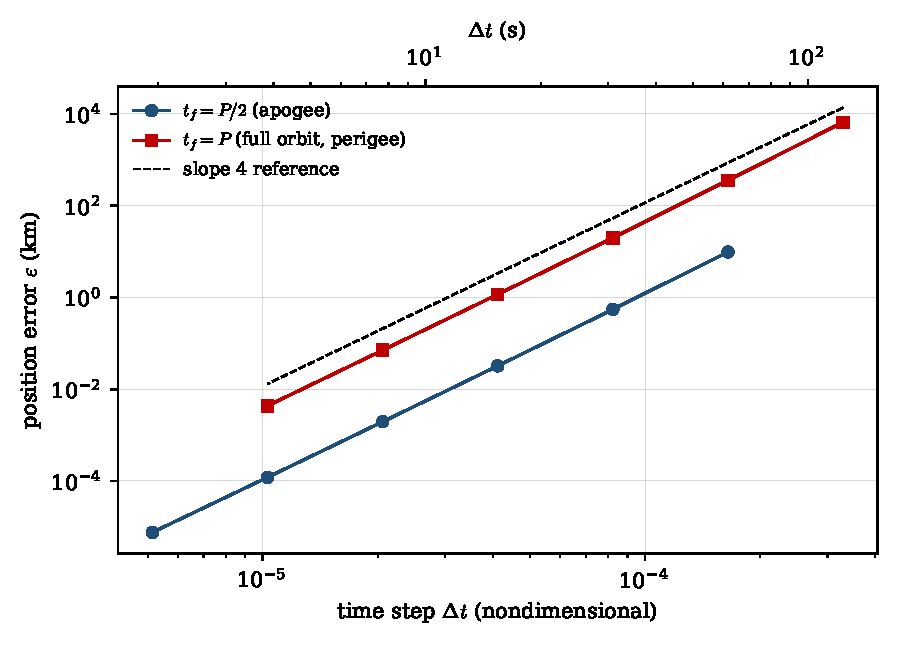
\includegraphics[width=0.62\textwidth]{figures/verify_kepler.pdf}
\caption{RK4 position error against the exact two-body solution ($\mu = 0$, $e = 0.97$, perigee at $r_0$) after half an orbit and after a full orbit. Both converge at fourth order.}
\label{fig:kepler}
\end{figure}

\paragraph{Published periodic orbit.} Because $\mu = 0$ multiplies every Moon term by zero, the two-body test cannot detect a mistake in those terms. We therefore also integrate a distant retrograde orbit from JPL's Earth--Moon CR3BP catalog~\cite{jpl_periodic} (first member of the DRO family; $\mu = 0.01215058561$, period $6.3052$, closest approach $14{,}300$\,km from Earth's center), which must return to its initial state after exactly one period. The Jacobi constant computed from the published state agrees with the catalog value to 13 digits, and the closure error falls at observed orders $4.03$--$4.13$ (Figure~\ref{fig:jpl}). An error in $\bff$ would make the closure error level off at a nonzero value instead.

\paragraph{Jacobi constant.} Along the nominal free return, from TLI to entry interface, the maximum drift $\max_k |C(t_k) - C(0)|$ falls at observed orders $4.03$--$4.22$ (Figure~\ref{fig:jpl}), reaching $3.5\times10^{-8}$ at the study time step.

\begin{figure}[t]
\centering
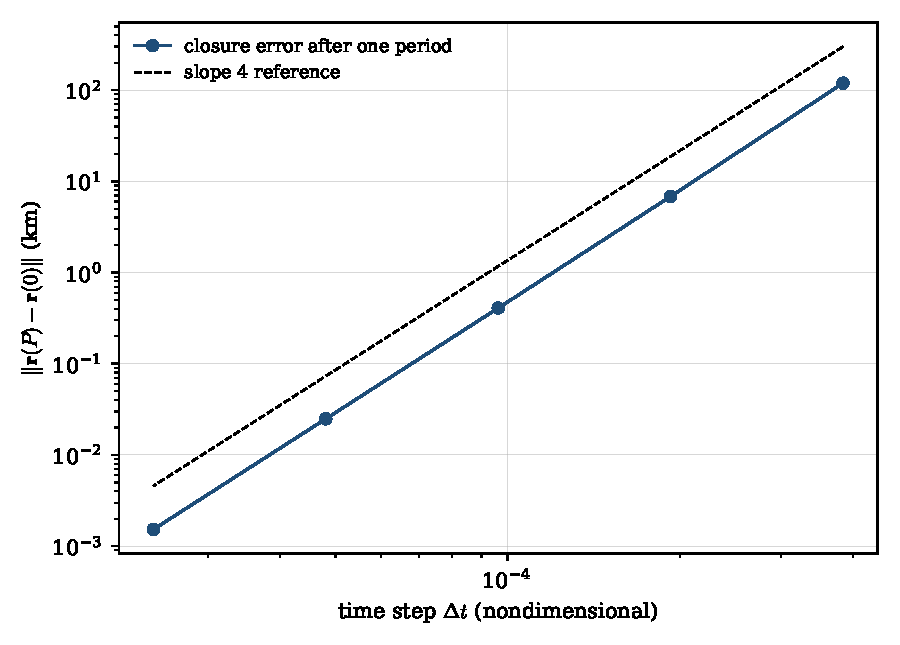
\includegraphics[width=0.49\textwidth]{figures/verify_jpl_dro.pdf}\hfill
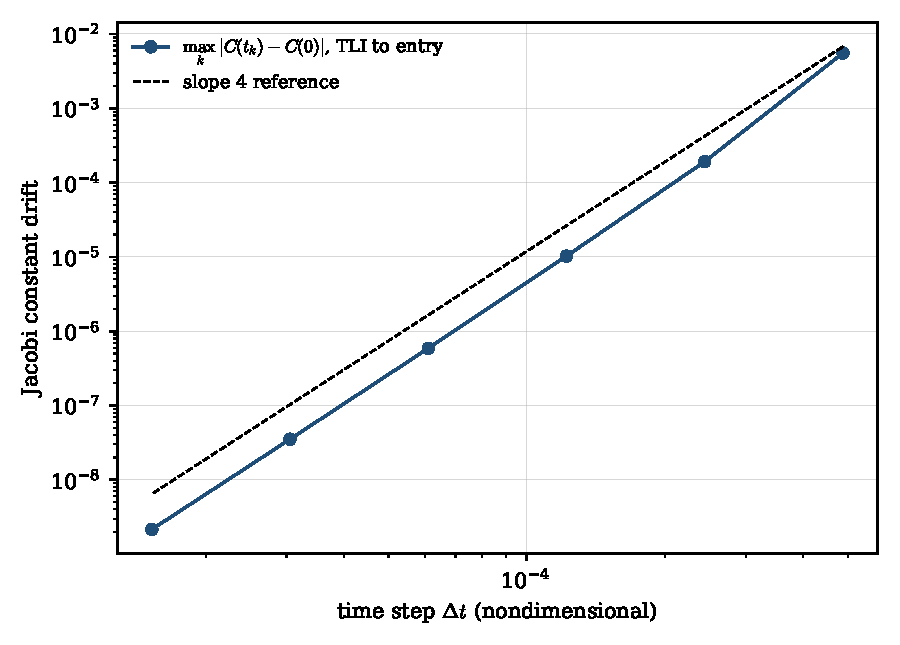
\includegraphics[width=0.49\textwidth]{figures/verify_jacobi.pdf}
\caption{Left: closure error of the JPL distant retrograde orbit after one published period. Right: Jacobi-constant drift along the nominal free return. Both decrease at fourth order.}
\label{fig:jpl}
\end{figure}

\paragraph{Convergence study.} The self-convergence study in \texttt{FreeReturnTrajectory.ipynb} integrates the nominal to $t_f = 1.7$ (just before entry interface) and compares the full state against a reference with $\Delta t = t_f/2^{17}$, for $\Delta t = t_f/2^{12}$ to $t_f/2^{16}$. The observed orders are $4.50$, $4.21$, $4.12$, $4.14$. At $\Delta t \approx 10^{-3}$ the trajectory never returns to Earth, so that step lies outside the asymptotic range.

\subsection{Selecting simulation parameters}

The time step must make the numerical error in $\gEI$ negligible compared with both (i) the corridor width, $2.15^\circ$, and (ii) the change in $\gEI$ produced by the smallest injection error we resolve, $\approx 0.1$\,mm/s. At the nominal $d\gEI/d(\Delta v) = -0.14^\circ$ per mm/s, so requirement (ii) is $0.014^\circ$ and requirement (i), $1\%$ of the corridor, is $0.0215^\circ$. Figure~\ref{fig:dt} plots the $\gEI$ error against $\Delta t$, measured against a reference with $\Delta t = 1.9\times10^{-6}$. The error falls at observed orders $4.39$--$4.03$, which also confirms that the event location keeps fourth-order accuracy. We use $\Delta t = 3.05\times 10^{-5}$ ($11.4$\,s), where the $\gEI$ error is $2.3\times10^{-4}$ degrees, about $60\times$ below the tighter requirement, at about $2$\,s per run. This $\Delta t$ is used for all results in Section~\ref{sec:results}.

\begin{figure}[t]
\centering
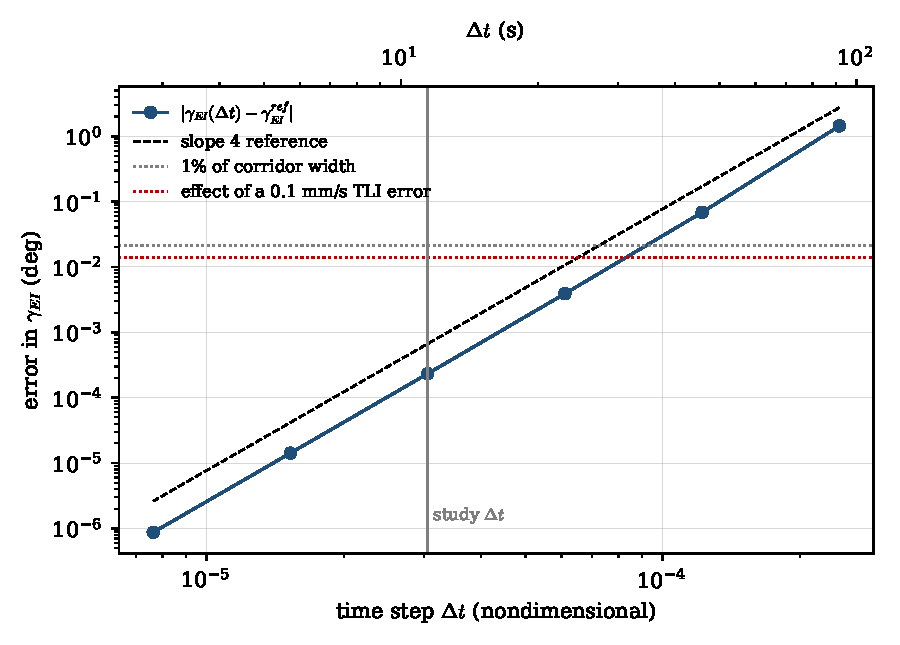
\includegraphics[width=0.62\textwidth]{figures/select_dt.pdf}
\caption{Error in the entry flight-path angle against time step, with the two accuracy requirements. The vertical line marks the study time step.}
\label{fig:dt}
\end{figure}

% =====================================================================
\section{Results}
\label{sec:results}
% =====================================================================

\subsection{Procedure}

\begin{enumerate}[leftmargin=2em]
  \item \textbf{Nominal.} Retarget the free return to $\gEI = -6.52^\circ$; report $\Delta v$, $\varphi$, perilune altitude, time of flight, and $C$.
  \item \textbf{Q1a.} Sweep $\delta(\Delta v)$ over $\pm 20$\,mm/s with $\varphi$ fixed; record $\gEI$ (or impact/no return).
  \item \textbf{Q1b.} Sweep $\delta t$ over $\pm 2$\,s with $\Delta v$ fixed; record $\gEI$.
  \item \textbf{Q1 tolerances.} Root-find the $\delta(\Delta v)$ and $\delta t$ at which $\gEI$ reaches $-5.25^\circ$ and $-7.4^\circ$, including any shallow/steep asymmetry.
  \item \textbf{Q2.} For representative injection errors well outside the corridor (e.g.\ $\delta(\Delta v) = \pm 1$\,m/s), solve for the $\Delta v_c$ restoring $\gEI = -6.52^\circ$ at 15--20 correction times $t_c$ between shortly after TLI and about one day before entry.
\end{enumerate}

\subsection{Planned figures}

\begin{itemize}[leftmargin=2em]
  \item Nominal free-return trajectory in the rotating frame, with perilune and entry interface marked (context). \todo{}
  \item $\gEI$ vs.\ $\delta(\Delta v)$, corridor shaded (answers Q1a). \todo{}
  \item $\gEI$ vs.\ $\delta t$, corridor shaded (answers Q1b). \todo{}
  \item Table of allowable TLI magnitude and timing errors (answers Q1). \todo{}
  \item $\Delta v_c$ vs.\ $t_c$ for each injection error, lunar closest approach marked (answers Q2). \todo{}
\end{itemize}

\subsection{Scope and limitations}

The corridor is used as a targeting criterion; atmospheric flight, heating, skip dynamics, and entry guidance are outside the model. The planar, circular CR3BP neglects the Moon's inclination and eccentricity, solar gravity, and $J_2$, so absolute values will differ from a real mission; the orders of magnitude of the sensitivities and the trends in correction cost are the transferable results. Burns are impulsive, and magnitude and timing errors are studied separately.

% =====================================================================
\section{Contributions}
% =====================================================================

\todo{each member's role and estimated percentage contribution; every member must contribute to at least one of Sections 1--4.}

% =====================================================================
\section{Reproducibility}
% =====================================================================

All code is available at https://github.com/boyakhil978/FreeReturnTrajectory. The repository separates the numerical method from the studies that use it:
\begin{itemize}[leftmargin=2em]
  \item \texttt{cr3bp.py}: right-hand side $\bff(\bu)$, initial-condition builder, $\gEI$, and $C$;
  \item \texttt{rk4.py}: fixed-step marcher \texttt{u, times = rk4(f, u0, t\_end, dt)} and event location;
  \item \texttt{verify\_*.py}: Kepler, Jacobi, convergence, and time-step selection studies;
  \item \texttt{study\_q1.py}, \texttt{study\_q2.py}: results figures;
  \item \texttt{README.md}: instructions to reproduce every figure.
\end{itemize}

% =====================================================================
\section*{Acknowledgments}
% =====================================================================

\todo{overview of how generative AI was used: ideation, method selection and justification, implementation and testing, figures and results.}

% =====================================================================
\begin{thebibliography}{9}
% =====================================================================

\bibitem{nasa_apollo13}
NASA, ``Houston, We've Had a Problem,'' NASA History.
\url{https://www.nasa.gov/history/houston-weve-had-a-problem/}

\bibitem{afj_day5}
Apollo 13 Flight Journal, ``Day 5: Wobbles and Bursts,'' \emph{Apollo Flight Journal}. Corridor at approx.\ 108:52 MET; $-6.52^\circ$ target at approx.\ 109:30 MET.
\url{https://apollojournals.org/afj/ap13fj/20day5-wobblesandbursts.html}

\bibitem{rea_orion}
J.~R.~Rea, ``Orion Entry Performance-Based Center-of-Gravity Box,'' AIAA Guidance, Navigation, and Control Conference, Toronto, 2010, JSC-CN-19821.
\url{https://ntrs.nasa.gov/citations/20100005142}

\bibitem{rea_artemis1}
J.~R.~Rea, L.~McNamara, and M.~Kane, ``Orion Artemis I Entry Performance,'' AAS Paper 24-174, NASA Johnson Space Center, 2024.
\url{https://ntrs.nasa.gov/citations/20240000024}

\bibitem{jpl_periodic}
JPL Solar System Dynamics, ``Three-Body Periodic Orbits,'' Earth--Moon system, DRO family.
\url{https://ssd.jpl.nasa.gov/tools/periodic_orbits.html}

\bibitem{szebehely}
V.~Szebehely, \emph{Theory of Orbits: The Restricted Problem of Three Bodies}, Academic Press, 1967.

\end{thebibliography}

\end{document}